\documentclass[12pt]{jarticle}
\usepackage{TUSIReport}
\usepackage{otf}
\usepackage[dvipdfmx]{graphicx}
\usepackage[dvipdfmx]{color}
\usepackage{amsmath}
\usepackage{amssymb}
\usepackage{color}
\usepackage{hhline}
\usepackage{fancybox,ascmac}
\usepackage{multirow}
\usepackage{url}
\usepackage{bm}
\usepackage{listings,jlisting}
\lstdefinestyle{log}{
    frame={tblr},
    basicstyle={\footnotesize},
    tabsize={4},
}
\lstdefinestyle{lstcpp}{
    language={c++},
    backgroundcolor={\color[gray]{.85}},
    basicstyle={\small},
    identifierstyle={\small},
    commentstyle={\small\ttfamily \color[rgb]{0,0.5,0}},
    keywordstyle={\small\bfseries \color[rgb]{1,0,0}},
    ndkeywordstyle={\small},
    stringstyle={\small\ttfamily \color[rgb]{0,0,1}},
    frame={tb},
    breaklines=true,
    columns=[l]{fullflexible},
    numbers=left,
    xrightmargin=0zw,
    xleftmargin=3zw,
    numberstyle={\scriptsize},
    stepnumber=1,
    numbersep=1zw,
    morecomment=[l]{//}
}
\begin{document}
%%%%%%%%%%%%%%%%%%%%%%%%%%%%%%%%%%%%%%%%%%%%%%%%%%%%%%%%%%%%%%
% 表紙を出力する場合は,\提出者と\共同実験者をいれる
% \提出者{科目名}{課題名}{提出年}{提出月}{提出日}{学籍番号}{氏名}
% \共同実験者{一人目}{二人目}{..}{..}{..}{..}{..}{八人目}
%%%%%%%%%%%%%%%%%%%%%%%%%%%%%%%%%%%%%%%%%%%%%%%%%%%%%%%%%%%%%%
\提出者{情報工学実験2}{実験テーマ3 情報通信シミュレーション}{2020}{12}{7}{4619055}{辰川力駆}
\共同実験者{}{}{}{}{}{}{}{}

%%%%%%%%%%%%%%%%%%%%%%%%%%%%%%%%%%%%%%%%%%%%%%%%%%%%%%%%%%%%%%
% 表紙を出力しない場合は,以下の「\表紙出力」をコメントアウトする
%%%%%%%%%%%%%%%%%%%%%%%%%%%%%%%%%%%%%%%%%%%%%%%%%%%%%%%%%%%%%%
\表紙出力

%%%%%%%%%%%%%%%%%%%%%%%%%%%%%%%%%%%%%%%%%%%%%%%%%%%%%%%%%%%%%%
% 以下はレポート本体である.別途 TeXファイルを作成し \input 使っても良い
%%%%%%%%%%%%%%%%%%%%%%%%%%%%%%%%%%%%%%%%%%%%%%%%%%%%%%%%%%%%%%

\section{実験概要}
 (7,4)ハミング符号による符号化、復号を行うプログラムを作成して、
ハミング符号の特徴を理解する。

\section{実験手順}
\begin{enumerate}
    \item 4ビットの情報 $\boldsymbol{w}$ を生成
    \item 生成多項式 $g(x)$ を用いて符号化
    \item 1ビットの雑音を付与する
    \item 受信語 $\boldsymbol{y}$ と検査行列 $H$ からシンドローム $\boldsymbol{s}$ を計算
    \item シンドロームから誤り位置を推定する
    \item 推定語 $\hat{\boldsymbol{x}}$ を求め、もとの $\boldsymbol{x}$ と値を比較する
\end{enumerate}

\section{実験結果}

ソースコードは付録に記述した。
そのソースコードを実行した結果を下記に示す。

\begin{figure}[h]
    \begin{center}
        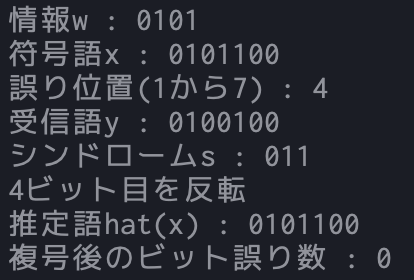
\includegraphics[scale=0.8]{kadai3_2_1.png}
    \end{center}
    \caption{$情報=0101$、$誤り位置=4$の実行結果}
\end{figure}
\clearpage
\begin{figure}[h]
    \begin{center}
        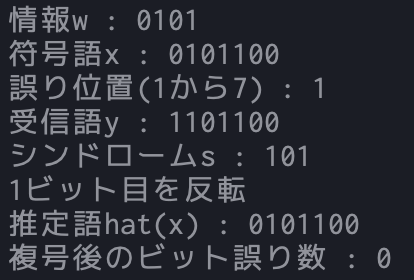
\includegraphics[scale=0.8]{kadai3_2_2.png}
    \end{center}
    \caption{$情報=0101$、$誤り位置=1$の実行結果}
\end{figure}

\section{検討}
\subsection{課題1}
\begin{shadebox}
    シミュレーションによるビット誤り率と理論値が
    ほぼ同じ値になるにはどの程度のシミュレーション回数を実行する必要があるか。
\end{shadebox}


\subsection{課題2}
\begin{shadebox}
    $\epsilon$を非常に小さくした場合、これはどうなるか。
\end{shadebox}

\clearpage

\subsection{課題3}
\begin{shadebox}
    $\rm{rand()}$と$\rm{MT}$の違いは何か。
\end{shadebox}

\clearpage
% 付録
\appendix
\section{付録}
\begin{lstlisting}[style = lstcpp,caption=kadai3\_2.cpp]
    //4619055 辰川力駆
    #include <random> // 乱数生成
    #include <stdio.h>
    #include <iostream>
    #include <iomanip>
    
    using namespace std;
    
    #define N 7 //符号化後のビット数
    #define K 4 //デジタル情報の分けるブロックのビット数
    
    int main()
    {
        int w[K] = {0, 1, 0, 1}; //4ビットの情報w
        int x[N];                //7ビットの符号語x
        int y[N];                //7ビットの受信語y
        int ErrorPosition;       //誤り位置(1から7)
        int s[3];                //シンドロームs
        int EstimationPosition;  //誤り位置推定場所
        int cnt = 0;             //復号後のビット誤り数
    
        cout << "情報w : ";
        for (int i = 0; i < K; i++)
        {
            cout << w[i];
        }
        cout << endl;
    
        for (int i = 0; i < K; i++)
        {
            x[i] = w[i];
        }
        x[N - K + 1] = w[0] ^ w[1] ^ w[2];
        x[N - K + 2] = w[1] ^ w[2] ^ w[3];
        x[N - K + 3] = w[0] ^ w[1] ^ w[3];
        cout << "符号語x : ";
        for (int i = 0; i < N; i++)
        {
            cout << x[i];
        }
        cout << endl;
    
        cout << "誤り位置(1から7) : ";
        cin >> ErrorPosition;
    
        cout << "受信語y : ";
        for (int i = 0; i < N; i++)
        {
            y[i] = x[i];
            if (i == ErrorPosition - 1)
            {
                y[i] = x[i] ^ 1; //誤り位置は反転する
            }
            cout << y[i];
        }
        cout << endl;
    
        s[0] = y[0] ^ y[1] ^ y[2] ^ y[4];
        s[1] = y[1] ^ y[2] ^ y[3] ^ y[5];
        s[2] = y[0] ^ y[1] ^ y[3] ^ y[6];
        cout << "シンドロームs : ";
        for (int i = 0; i < 3; i++)
        {
            cout << s[i];
        }
        cout << endl;
    
        int point = 0;
        for (int i = 0; i < 3; i++)
        {
            point += s[i] * pow(2, 2 - i);
        }
        switch (point)
        {
        case 5:
            EstimationPosition = 1;
            break;
        case 7:
            EstimationPosition = 2;
            break;
        case 6:
            EstimationPosition = 3;
            break;
        case 3:
            EstimationPosition = 4;
            break;
        case 4:
            EstimationPosition = 5;
            break;
        case 2:
            EstimationPosition = 6;
            break;
        case 1:
            EstimationPosition = 7;
            break;
        default:
            EstimationPosition = -1;
            break;
        }
    
        if (EstimationPosition == -1)
        {
            cout << "誤りはなし" << endl;
        }
        else
        {
            cout << EstimationPosition << "ビット目を反転" << endl;
        }
    
        y[EstimationPosition - 1] = y[EstimationPosition - 1] ^ 1;
        cout << "推定語hat(x) : ";
        for (int i = 0; i < N; i++)
        {
            cout << y[i];
        }
        cout << endl;
    
        for (int i = 0; i < N; i++)
        {
            cnt += x[i] ^ y[i];
        }
        cout << "複号後のビット誤り数 : " << cnt << endl;
    
        return 0;
    }
    
\end{lstlisting}

%%%%%%%%%%%%%%%%%%%%%%%%%%%%%%%%%%%%%%%%%%%%%%%%%%%%%%%%%%%%%%
\end{document}